\documentclass[a4paper, 11pt]{report}

\usepackage[french]{babel}
\usepackage[a4paper]{geometry}
\usepackage{amsmath}
\usepackage{amsthm}
\usepackage{amssymb}
\usepackage{mathtools}
\usepackage{enumitem}
\usepackage{graphicx}
\usepackage[hidelinks]{hyperref}


\newtheorem*{theorem}{Théorème}
\newtheorem*{corollary}{Corollaire}

\theoremstyle{definition}
\newtheorem*{motivation}{Motivation}
\newtheorem*{hypothesis}{Hypothèses}
\newtheorem*{result}{Résultat}
\newtheorem*{definition}{Définition}
\newtheorem*{idea}{Idée}

\theoremstyle{remark}
\newtheorem*{terminology}{Terminologie}
\newtheorem*{note}{Note}
\newtheorem*{remark}{Remarque}
\newtheorem*{example}{Exemple}
\newtheorem*{illustration}{Illustration}

\newcommand{\N}{\mathbb{N}}
\newcommand{\Z}{\mathbb{Z}}
\newcommand{\R}{\mathbb{R}}
\newcommand{\Cx}{\mathbb{C}}
\newcommand{\dd}{\mathrm{d}}
\newcommand{\dl}{\mathrm{d}\ell}
\newcommand{\dt}{\mathrm{d}t}
\newcommand{\dx}{\mathrm{d}x}
\newcommand{\dy}{\mathrm{d}y}
\newcommand{\dz}{\mathrm{d}z}
\newcommand{\dal}{\mathrm{d}\alpha}
\newcommand{\dth}{\mathrm{d}\theta}
\newcommand{\dxi}{\mathrm{d}\xi}
\newcommand{\TF}{\mathfrak{F}}
\newcommand{\TFi}{\TF^{-1}}
\newcommand{\ostpi}{\frac{1}{\sqrt{2 \pi}}} % one (over) sqrt of two Pi
\newcommand{\oipi}{\frac{1}{2 \pi i}} % one (over) i times two Pi
\newcommand{\cd}{\cdot}
\newcommand{\Rep}{\operatorname{Re}}
\newcommand{\Imp}{\operatorname{Im}}
\newcommand*\conj[1]{\overline{#1}}
\newcommand*\module[1]{\left|#1\right|}
\newcommand{\Arctg}{\textrm{Arctg}\,}
\newcommand{\inte}{\textrm{int}\,}
\newcommand{\rot}{\textrm{rot}\,}
\newcommand{\bord}{\partial}
\newcommand*\adh[1]{\conj{\inte #1}}
\newcommand{\Res}{\textrm{Rés}}


\title{\textbf{Analyse IV} \\
Transcript du cours du Pr. Michel \bsc{Cibils}}
\author{Robin \bsc{Mamié}}
\date{Printemps 2018}


\begin{document}

\maketitle

\tableofcontents

% !TeX spellcheck = fr_FR
\chapter{Transformées de Fourier}


\section{Introduction}


\subsection{Définitions et résultats préliminaires}

\begin{definition}
    Une fonction $f: \R \rightarrow \R$ est dite \textbf{T-périodique} s'il existe $T > 0$ tel que $f(x + T) = f(x) \enspace \forall x \in \R$.
    
    L'intervalle $[0, T]$ caractérise complètement la fonction.
\end{definition}


\begin{definition}[14.1.i, p.103]

    Une fonction $f: \R \rightarrow \R$ est dite \textbf{continue par morceaux} sur l'intervalle $[a, b]$ s'il existe des points $ \{x\}_{i = 0}^{n + 1} \subset [a, b]$ avec $a = x_0 < x_1 < \cdots < x_n < x_{n + 1} = b$ tels que pour $i = 0, 1, \ldots, n$ on ait:
    
    \begin{enumerate}

        \item
        $f$ est continue sur chaque intervalle ouvert $]x_i, x_{i + 1}[$

        \item
        la limite à droite $f(x_i + 0) := \lim\limits_{\substack{t \rightarrow x_i \\ t > x_i}} f(t)$ et la limite à gauche $f(x_{i + 1} - 0) := \lim\limits_{\substack{t \rightarrow x_i \\ t < x_i}} f(t)$ existent et sont finies.

    \end{enumerate}

\end{definition}


\begin{terminology}
    On dit qu'une fonction T-périodique est continue par morceaux si elle l'est sur l'intervalle $[0, T]$ qui la caractérise.
\end{terminology}


\begin{definition}[14.2, p.104]
    Soit $f: \R \rightarrow \R$ une fonction T-périodique continue par morceaux.
    Pour $N \in \mathbb{N}$, la \textbf{série de Fourier partielle d'ordre N} de $f$ est:
    
    \[
    F_N f(x) = \sum_{n = -N}^{N} c_n e^{i \frac{2 \pi n}{T} x}
    \]
    
    où les \textbf{coefficients de Fourier} $c_n$ sont des nombres complexes donnés par:
    
    \[
    c_n = \frac{1}{T} \int_{0}^{T} f(x) e^{-i \frac{2 \pi n}{T} x} \dx
    \]
    
    On appelle \textbf{série de Fourier de f} (en notation complexe) la limite lorsque $N \longrightarrow \infty$ de la série de $F_N f(x)$.
    On écrit:
    
    \[ F f(x) := \lim_{N \rightarrow +\infty} F_N f(x) = \sum_{-\infty}^{\infty} c_n e^{i \frac{2 \pi n}{T} x} \]
\end{definition}


\begin{theorem}[de Dirichlet -- Résultat de convergence; 14.3, p.104]
    Soit $f: \R \rightarrow \R$ une fonction T-périodique telle que $f$ et $f'$ soient continues par morceaux.
    Alors $\forall x \in \R$:
    
    \[
    F f(x) = \lim\limits_{N \rightarrow \infty} F_N f(x) \textrm{ existe et } F f(x) = \frac{f(x + 0) + f(x - 0)}{2}
    \]
    
    En particulier, si $f$ est continue en $x$, alors $f(x + 0) = f(x - 0) = f(x)$ et on a $F f(x) = f(x)$.
\end{theorem}


\begin{note}
    Utilisation de la formule d'Euler $e^{ix} = \cos x + i \sin x$ \textit{(cf. ex. 1-2, série 1)}.
\end{note}


\subsection{Motivation}

\begin{description}

    \item[Série de Fourier]
    développement des fonctions \textit{périodiques} comme somme infinie de fonctions trigonométriques.
    
    \item[Transformée de Fourier]
    étude de fonctions \textit{non} périodiques.

\end{description}


\begin{idea}
    Soit $T > 0$ et $f_T$ une fonction T-périodique définie par
    
    \[
    f_T (x) =
    \left \{
    \begin{array}{r c l}
        0 & \mathrm{si} & x \in \enspace ]-\frac{T}{2}, -1[ \\
        1 & \mathrm{si} & x \in [-1, 1] \\
        0 & \mathrm{si} & x \in \enspace ]1, \frac{T}{2}[ \\
    \end{array}
    \right .
    \]
    
    Lorsque la période $T \rightarrow \infty$, on a:
    
    \[
    \lim_{T \rightarrow \infty} f_T (x) = f(x) =
    \left \{
    \begin{array}{r c l}
        1 & \mathrm{si} & x \in [-1, 1] \\
        0 & \mathrm{si} & x \notin [-1, 1] \\
    \end{array}
    \right .
    \]
    
    qui n'est plus une fonction périodique.
    
\end{idea}


\begin{idea}
    considérer des fonctions comme limites de fonctions périodiques dont la période $T$ tend vers $+\infty$.
\end{idea}


\subsection{Raisonnement heuristique}

Soit $f_T: \R \rightarrow \R$ une fonction \textit{continue}, T-périodique telle que $f'_T$ soit continue par morceaux.
Alors la série de Fourier de $f_T$ est:

\[
F f_T(y) = \sum_{-\infty}^{+\infty} c_n e^{i \frac{2 \pi n}{T} y}
\]

pour $y \in \R$, où

\[
c_n = \frac{1}{T} \int_{0}^{T} f_T(x) e^{-i \frac{2 \pi n}{T} x} \dx
= \frac{1}{T} \int_{-\frac{T}{2}}^{\frac{T}{2}} f_T(x) e^{-i \frac{2 \pi n}{T} x} \dx
\]

En écrivant
$\Delta \alpha = \frac{2 \pi}{T}$
et
$\alpha_n = n \cdot \Delta \alpha$,
on a
$\frac{1}{T} = \frac{\Delta \alpha}{2 \pi}$.

\[
c_n =
\frac{\Delta \alpha}{2 \pi}
\int_{-\frac{T}{2}}^{\frac{T}{2}} f_T(x) e^{-i \alpha_n x} \dx
\]

\[
\Rightarrow
F f_T(y) =
\sum_{-\infty}^{+\infty}
\left[
\frac{\Delta \alpha}{2 \pi}
\int_{-\frac{T}{2}}^{\frac{T}{2}}
f_T(x) e^{-i \alpha_n x} \dx
\right]
e^{i \alpha_n y}
\]

Échange de la somme infinie et de l'intégrale:

\[
F f_T(y) =
\frac{1}{2 \pi}
\int_{-\frac{T}{2}}^{\frac{T}{2}}
f_T(x)
\left[
\Delta \alpha
\sum_{-\infty}^{+\infty}
e^{-i \alpha_n (x - y)}
\right]
\dx
\]

On découvre une somme de Riemann qui permet de définir une intégrale.
En effet:

\[
\Delta \alpha \sum_{-\infty}^{+\infty}
e^{-i \alpha_n (x - y)}
\underbrace{=}_{\Delta\alpha = \alpha_n - \alpha_{n - 1}}
\sum_{-\infty}^{+\infty}
e^{-i \alpha_n (x - y)} (\alpha_n - \alpha_{n - 1})
\]

\[
=
\int_{-\infty}^{+\infty}
e^{-i \alpha (x - y)}
\dal
\]

Donc on obtient:

\begin{align*}
F f_T(y) &=
\frac{1}{2 \pi}
\int_{-\frac{T}{2}}^{\frac{T}{2}}
f_T(x)
\left[
\int_{-\infty}^{+\infty}
e^{-i \alpha (x - y)}
\dal
\right]
\dx
\\&=
\frac{1}{\sqrt{2 \pi}}
\int_{-\infty}^{+\infty}
\left[
\frac{1}{\sqrt{2 \pi}}
\int_{-\frac{T}{2}}^{\frac{T}{2}}
f_T(x) e^{-i \alpha x}
\dx
\right]
e^{i \alpha y}
\dal
\end{align*}

Comme $f_T$ est continue, alors on a $f_T(y) = F f_T(y)$ et donc lorsque $T$ tend vers $+\infty$, on a
$\lim\limits_{T \rightarrow +\infty} f_T(y) =
\lim\limits_{T \rightarrow +\infty} F f_T(y) \iff
f(y) = \lim\limits_{T \rightarrow +\infty} F f_T(y)$.

\[
\iff
f(y) =
\frac{1}{\sqrt{2 \pi}}
\int_{-\infty}^{+\infty}
\underbrace{
\left[
\frac{1}{\sqrt{2 \pi}}
\int_{-\infty}^{+\infty}
f(x) e^{-i \alpha x}
\dx
\right]
}_{\substack{
\textrm{Nouvelle fonction qui dépend de la}\\
\textrm{variable $\alpha$, qui est appelée la}\\
\textrm{transformée de Fourier de $f$ et}\\
\textrm{notée $\TF(f)$ ou $\hat{f}$}
}}
e^{i \alpha y}
\dal
\]

On écrit:

\[
\TF(f)(\alpha) = \hat{f}(\alpha) =
\frac{1}{\sqrt{2 \pi}}
\int_{-\infty}^{+\infty}
f(x) e^{-i \alpha x}
\dx
\]

\begin{remark}
    On a que:
    
    \[
    f(y) =
    \frac{1}{\sqrt{2 \pi}}
    \int_{-\infty}^{+\infty}
    \hat{f}(\alpha)
    e^{i \alpha y}
    \dal
    \]
\end{remark}



\section{Transformée de Fourier d'une fonction}


\subsection{Définition}

\begin{definition}[15.1, p.113]
    Soit $f: \R \rightarrow \R$ une fonction continue par morceaux et telle que $\int_{-\infty}^{+\infty} | f(x) | \dx < \infty$.
    
    La \textbf{transformée de Fourier} de $f$ est la fonction notée $\TF(f)$ ou $\hat{f}: \R \rightarrow \C$ définie par:
    
    \[
    \alpha \longmapsto
    \TF(f)(\alpha) = \hat{f}(\alpha) =
    \frac{1}{\sqrt{2 \pi}}
    \int_{-\infty}^{+\infty}
    f(x) e^{-i \alpha x}
    \dx
    \]
\end{definition}


\subsection{Exemples}

\begin{example}
    Calculer la transformée de Fourier de la fonction:
    
    \[
    f:
    \begin{array}{r c l}
        \R & \rightarrow & \R_+^* \\
        x  & \mapsto & f(x) = e^{-|x|} =
        \left \{
        \begin{array}{r c l}
            e^{-x} & \textrm{si} & x \geq 0 \\
            e^x    & \textrm{si} & x < 0
        \end{array}
        \right.
    \end{array}
    \]
    
    \begin{align*}
    \hat{f}(\alpha) & =
    \frac{1}{\sqrt{2 \pi}}
    \int_{-\infty}^{+\infty}
    f(x)
    e^{-i \alpha x}
    \dx
    =
    \frac{1}{\sqrt{2 \pi}}
    \int_{-\infty}^{+\infty}
    e^{-|x|}
    e^{-i \alpha x}
    \dx
    \\&=
    \frac{1}{\sqrt{2 \pi}}
    \left[
    \int_{-\infty}^{0}
    e^{x}
    e^{-i \alpha x}
    \dx
    +
    \int_{0}^{+\infty}
    e^{-x}
    e^{-i \alpha x}
    \dx
    \right]
    \\&=
    \frac{1}{\sqrt{2 \pi}}
    \left[
    \int_{-\infty}^{0}
    e^{(1 - i \alpha) x}
    \dx
    +
    \int_{0}^{+\infty}
    e^{-(1 + i \alpha) x}
    \dx
    \right]
    \\&=
    \frac{1}{\sqrt{2 \pi}}
    \left[
    \left.
    \frac{e^{(1 - i \alpha) x}}
    {1 - i \alpha}
    \right|_{-\infty}^0
    -
    \left.
    \frac{e^{-(1 + i \alpha) x}}
    {1 + i \alpha}
    \right|_0^{+\infty}
    \right]
    \\&=
    \frac{1}{\sqrt{2 \pi}}
    \left[
    \frac{1}
    {1 - i \alpha}
    \left(
    1 - \lim\limits_{x \rightarrow -\infty} e^{(1 - i \alpha) x}
    \right)
    \right.
    -
    \left.
    \frac{1}
    {1 + i \alpha}
    \left(
    \lim\limits_{x \rightarrow + \infty} e^{-(1 + i \alpha) x} - 1
    \right)
    \right]
    \\&=
    \frac{1}{\sqrt{2 \pi}}
    \left(
    \frac{1}{1 - i \alpha}
    +
    \frac{1}{1 + i \alpha}
    \right)
    \\&=
    \frac{1}{\sqrt{2 \pi}}
    \frac{1 + i \alpha + 1 - i \alpha}
    {(1 - i \alpha) (1 + i \alpha)}
    =
    \frac{1}{\sqrt{2 \pi}}
    \frac{2}{1 + \alpha^2}
    \end{align*}
    
    \textbf{Résultat:}
    
    \[
    \hat{f}:
    \begin{array}{r c l}
    \R & \rightarrow & \R_+^* \\
    \alpha & \mapsto & \hat{f}(\alpha) =
    \sqrt{\frac{2}{\pi}} \frac{1}{1 + \alpha^2}
    \end{array}
    \]
\end{example}


\begin{remark}
    Pour calculer
    $\lim\limits_{x \rightarrow -\infty} e^{(1 - i \alpha) x}$:
    
    \begin{align*}
    \left|e^{(1 - i \alpha) x}\right|
    &= \left|e^{- i \alpha x} e^x\right|
    = \underbrace{\left|e^{- i \alpha x}\right|}_{= 1} \left|e^x\right|
    = e^x\\
    \Rightarrow \lim\limits_{x \rightarrow -\infty} \left|e^{(1 - i \alpha) x}\right|
    &= \lim\limits_{x \rightarrow -\infty} e^x
    = 0\\
    \Rightarrow \lim\limits_{x \rightarrow -\infty} e^{(1 - i \alpha) x}
    &= 0 + i0
    = 0
    \end{align*}
    
    On a aussi $\lim\limits_{x \rightarrow +\infty} e^{-(1 + i \alpha) x} = 0$.
\end{remark}


\begin{example}
    Soit la fonction 
    
    \[
    f:
    \begin{array}{r c l}
    \R & \rightarrow & \R \\
    x  & \mapsto & f(x) = 
    \left \{
    \begin{array}{r c l}
    1 & \textrm{si} & x \in [-1, 1] \\
    0   & \textrm{sinon} &
    \end{array}
    \right.
    \end{array}
    \]
    
    Calcul de la transformée de Fourier de $f$.
    
    \begin{align*}
    \hat{f}(\alpha) & =
    \frac{1}{\sqrt{2 \pi}}
    \int_{-\infty}^{+\infty}
    f(x)
    e^{-i \alpha x}
    \dx
    =
    \frac{1}{\sqrt{2 \pi}}
    \int_{-1}^{1}
    e^{-i \alpha x}
    \dx
    \\&\overbrace{=}^{\alpha \neq 0}
    -
    \frac{1}{\sqrt{2 \pi}}
    \left.
    \frac{e^{-i \alpha x}}{i \alpha}
    \right|_{-1}^{1}
    =
    \frac{1}{\sqrt{2 \pi}}
    \frac{e^{i \alpha} - e^{-i \alpha}}{i \alpha}
    \\&=
    \frac{2}{\sqrt{2 \pi}}
    \frac{1}{\alpha}
    \frac{e^{i \alpha} - e^{-i \alpha}}{2i}
    =
    \sqrt{\frac{2}{\pi}}
    \frac{\sin \alpha}{\alpha}
    \quad
    \text{si } \alpha \neq 0
    \end{align*}
    
    Pour $\alpha = 0$ :
    
    \begin{align*}
    \hat{f}(0) &=
    \frac{1}{\sqrt{2 \pi}}
    \int_{-\infty}^{+\infty}
    f(x)
    e^{-i 0 x}
    \dx
    =
    \frac{1}{\sqrt{2 \pi}}
    \int_{-1}^{1}
    \dx
    =
    \left.
    \frac{1}{\sqrt{2 \pi}}
    x
    \right|_{-1}^{1}
    =
    \sqrt{\frac{2}{\pi}}
    \end{align*}
    
    \textbf{Résultat:}
    
    \[
    \hat{f}:
    \begin{array}{r c l}
    \R & \rightarrow & \R \\
    \alpha & \mapsto & \hat{f}(\alpha) =
    \left\{
    \begin{array}{l c l}
    \sqrt{\frac{2}{\pi}}
    \frac{\sin \alpha}{\alpha} & \mathrm{si} & \alpha \neq 0\\
    \sqrt{\frac{2}{\pi}} & \mathrm{si} & \alpha = 0
    \end{array}
    \right.
    \end{array}
    \]
    
    On remarque que $\lim\limits_{\alpha \rightarrow 0} \hat{f}(\alpha) = \lim\limits_{\alpha \rightarrow 0} \sqrt{\frac{2}{\pi}} \frac{\sin \alpha}{\alpha} = \sqrt{\frac{2}{\pi}} = \hat{f}(0)$.
    
    $\implies \hat{f}$ est aussi continue en $\alpha = 0$.
    
    \textit{Autres exemples: ex. 3-4, série 1}
    
\end{example}



\section{Transformée de Fourier inverse}


\subsection{Définition}

\begin{definition}
    Soit $g: \R \rightarrow \C$ une fonction continue par morceaux telle que $\int_{-\infty}^{+ \infty} |g(t)| \dt < \infty$.
    La \textbf{transformée de Fourier inverse} de $g$ est notée:
    
    \[
    \TFi(g):
    \begin{array}{r c l}
    \R & \rightarrow & \C \\
    x & \rightarrow & \TFi(g)(x)
    \end{array}, \textrm{ où}
    \enspace
    \TFi(g)(x) =
    \frac{1}{\sqrt{2 \pi}} \int_{-\infty}^{+\infty} g(t) e^{itx} \dt.
    \]
\end{definition}


\subsection{Théorème de réciprocité (formule d'inversion)}

\begin{theorem}[15.3.i, p.115]
    Soit $f: \R \rightarrow \R$ une fonction telle que $f$ et $f'$ soient continues par morceaux avec $\int_{-\infty}^{+ \infty} |f(x)| dx < \infty$ et $\int_{-\infty}^{+ \infty} |\hat{f}(\alpha)| \dal < \infty$.
    Alors $\forall x \in \R$, on a:
    
    \[
    \TFi (\hat{f})(x) =
    \frac{1}{\sqrt{2 \pi}}\int_{-\infty}^{+ \infty} \hat{f}(\alpha) e^{i\alpha x}\dal =
    \frac{f(x+0)+f(x-0)}{2}
    \]
    
    En particulier si $f$ est continue en $x$, on a $\frac{1}{2}[f(x+0) + f(x-0)] = f(x)$ et alors:
    
    \[
    f(x) = \TFi (\hat{f})(x) =
    \frac{1}{\sqrt{2 \pi}}
    \int_{-\infty}^{+ \infty}
    \hat{f}(\alpha) e^{i\alpha x}
    \dal
    \]
    
    Autrement dit, on a $\TFi(\TF(f)) = f$.
    La transformée de Fourier peut être vue comme une \og transformation $\TF$ \fg{} inversible (une bijection) qui \og agit\fg{} sur la fonction $f$:
    
    \[
    f \enspace
    \xrightarrow{\enspace \TF \enspace}
    \enspace \hat{f} \enspace
    \xrightarrow{\TFi}
    \enspace f
    \]
\end{theorem}


\subsection{Exemple d'utilisation}

\begin{example}
    Soit $
    f:
    \begin{array}{r c l}
    \R & \rightarrow & \R_+^* \\
    x  & \mapsto & f(x) = e^{-|x|} =
    \left \{
    \begin{array}{r c l}
    e^{-x} & \textrm{si} & x \geq 0 \\
    e^x    & \textrm{si} & x < 0
    \end{array}
    \right.
    \end{array}
    $.
    
    La transformée de Fourier de $f$ est (\textit{exemple 1, §1.2.2})
    
    \[
    \hat{f}:
    \begin{array}{r c l}
    \R & \rightarrow & \R_+^* \\
    \alpha & \mapsto & \hat{f}(\alpha) =
    \sqrt{\frac{2}{\pi}} \frac{1}{1 + \alpha^2}
    \end{array}
    \]

    On remarque que $f'(x) =
    \left\{
    \begin{array}{r c l}
    -e^{-x} & \textrm{si} & x \geq 0 \\
    e^x    & \textrm{si} & x < 0
    \end{array}
    \right.$
    est continue par morceaux car:
    
    \[\lim\limits_{\substack{x \rightarrow 0 \\ x > 0}} f'(x) = -1 \textrm{ et } \lim\limits_{\substack{x \rightarrow 0 \\ x < 0}} f'(x) = 1\]
    
    De plus, $\int_{-\infty}^{+\infty} |\hat{f}|\dx = \sqrt{\frac{2}{\pi}} \int_{-\infty}^{+\infty} \frac{\dal}{1 + \alpha^2} \dal < \infty$.
    $f$ est continue $\forall x \in \R \implies$ en appliquant le \textit{théorème de réciprocité}, on a que $f(x) = \frac{1}{\sqrt{2 \pi}} \int_{-\infty}^{+\infty} \hat{f}(\alpha) e^{i\alpha x}$, i.e.:
    
    \[
    e^{-|x|} =
    \frac{1}{\sqrt{2 \pi}} \sqrt{\frac{2}{\pi}} \int_{-\infty}^{+\infty} \frac{e^{i\alpha x}}{1 + \alpha^2}\dal
    \quad \forall x \in \R
    \]
    
    En particulier, lorsque $x = 0$, on trouve:
    
   \[1 = \frac{1}{\pi} \int_{-\infty}^{+\infty} \frac{\dal}{1 + \alpha^2} \implies \int_{-\infty}^{+\infty} \frac{\dal}{1 + \alpha^2} = \pi.
   \]
    
    En particulier, lorsque $x = 1$, on trouve:
    
    \begin{align*}
    e^{-1} &=
    \frac{1}{\pi} \int_{-\infty}^{+\infty} \frac{e^{i \alpha}}{1 + \alpha^2}\dal =
    \frac{1}{\pi} \left[ \int_{-\infty}^{+\infty} \frac{\cos \alpha}{1 + \alpha^2} \dal +
    i \overbrace{\int_{-\infty}^{+\infty} \frac{\sin \alpha}{1 + \alpha^2} \dal}^{\substack{\textrm{fonction impaire} \\ \textrm{intégrée sur tout l'axe} \\ \textrm{réel } = \> 0}} \right]
    \\&\implies
    \int_{-\infty}^{+\infty} \frac{\cos \alpha}{1 + \alpha^2} \dal = \frac{\pi}{e}
    \end{align*}

\end{example}

\textbf{Conclusion:} Le \textit{théorème de réciprocité} permet de calculer la valeur d'intégrales généralisées.

\textit{Autre exemple: ex. 1, série 2}



\section{Propriétés de la transformée de Fourier}


On considère $f$ et $g: \R \rightarrow \R$ continues par morceaux telles que $\int_{-\infty}^{+\infty} |f(x)| \dx < \infty$ et $\int_{-\infty}^{+\infty} |g(x)| \dx < \infty$.
On note indifféremment $\TF(f) \doteq \hat{f}$ et $\TF(g) \doteq \hat{g}$ les transformées de Fourier de $f$ et de $g$.

\begin{note}
    Les prochains résultats sont décrits dans les \textbf{théorèmes 15.2 et 15.3} aux pages 113 à 115 du livre du cours.
\end{note}


\subsection{Continuité et linéarité}

\begin{itemize}
\item
$\TF(f)$ est continue $\forall \alpha \in \R$ et $\lim\limits_{\alpha \rightarrow \pm \infty} |\TF(f)(\alpha)| = 0$.
\item
$\TF$ linéaire: $\TF(af + bg) = a\,\TF(f) + b\,\TF(g) \quad \forall a,b \in \R$.
\end{itemize}


\subsection{Transformée de Fourier du produit de convolution}

\begin{definition}
    Le \textbf{produit de convolution} de deux fonctions $f$ et $g$ est la fonction notée $f \ast g: \R \rightarrow \R$ définie par:
    
    \[(f \ast g)(x) := \int_{-\infty}^{+\infty} f(x - t) g(t) \dt\]
\end{definition}

\begin{remark}
    On peut aussi écrire $(f \ast g)(x) := \int_{-\infty}^{+\infty} f(t') g(x - t') \dt'$, via un changement de variable.
\end{remark}

\textbf{Résultat:} on a que $\TF(f \ast g) = \sqrt{2\pi} \enspace \TF(f) \cdot \TF(g)$.

La transformée de Fourier du produit de convolution de deux fonctions est égale au \textbf{produit} des transformées de Fourier de chaque fonction.

\textit{Exemples: ex. 2-3, série 2}


\subsection{Transformée de Fourier de la dérivée d'une fonction}

Si de plus $f \in C^1(\R)$ et $\int_{-\infty}^{+\infty} |f'(x)| \dx < \infty$, alors on a :

\[\TF(f')(\alpha) = i\alpha \enspace \TF(f)(\alpha) \quad \forall \alpha \in \R\]

On écrit aussi $\widehat{f'}(\alpha) = i\alpha \enspace \hat{f}(\alpha)$.

La transformée de Fourier de la dérivée de $f$ s'obtient en \textbf{multipliant par} $i\alpha$ la transformée de Fourier de $f$.

Plus généralement, si $f\in C^n(\R)$ et $\int_{-\infty}^{+\infty} |f^{(k)}(x)| \dx < \infty$ pour $k=1,2,\ldots,n$, alors on a:

\[\TF(f^{(k)})(\alpha) = (i\alpha)^k \enspace \TF(f)(\alpha) \quad \forall \alpha \in \R, k = 1,2,\ldots,n\]

On écrit aussi $\widehat{f^{(k)}}(\alpha) = (i\alpha)^k \enspace \hat{f}(\alpha)$.

\textit{Exemple: ex.3, série 2}


\subsection{Décalage}

Si $a \in \R^*, b \in \R$ et $h(x) = e^{-ibx}f(ax)$, alors:

\[\TF(h)(\alpha) = \frac{1}{|a|} \TF(f)\left(\frac{\alpha + b}{a}\right)\]


\subsection{Identité de Plancherel}

Si de plus $\int_{-\infty}^{+\infty} [f(x)]^2 \dx < \infty$, alors on a:

\[\int_{-\infty}^{+\infty} [f(x)]^2 \dx = \int_{-\infty}^{+\infty} |\TF(f)(\alpha)|^2 \dal\]


\subsection{Transformée de Fourier en sinus et cosinus}

Si la fonction $f$ est paire (i.e. $f(-x) = f(x) \enspace \forall x \in \R$), alors on a:

\[
\TF(f)(\alpha) =
\sqrt{\frac{2}{\pi}}
\int_{0}^{+\infty} f(x)\cos(\alpha x) \dx
\]

qui est la transformée de Fourier en \textbf{cosinus} de $f$.

Si la fonction $f$ est impaire (i.e. $f(-x) = -f(x) \enspace \forall x \in \R$), alors on a:

\[
\TF(f)(\alpha) =
- i
\sqrt{\frac{2}{\pi}}
\int_{0}^{+\infty} f(x)\sin(\alpha x) \dx
\]

qui est la transformée de Fourier en \textbf{sinus} de $f$.

\textit{Exemples: ex.4, série 2 et ex.1, série 3}

\begin{remark}
    Si de plus $f'$ est continue par morceaux et $\int_{-\infty}^{+\infty} |\hat{f}(\alpha)| \dal < \infty$, alors, d'après le \textit{théorème de réciprocité}, on a:
    
    \begin{align*}
    f(x) &=
    \sqrt{\frac{2}{\pi}}
    \int_{0}^{+\infty} \hat{f}(\alpha)\cos(\alpha x) \dal
    \quad
    \textrm{ lorsque } f \textrm{ est paire}\\
    f(x) &=
    i
    \sqrt{\frac{2}{\pi}}
    \int_{0}^{+\infty} \hat{f}(\alpha)\sin(\alpha x) \dal
    \quad
    \textrm{ lorsque } f \textrm{ est impaire}\\
    \end{align*}
\end{remark}


\section{Esquisse de démonstrations de quelques propriétés}

\subsection{Transformée de Fourier de la dérivée d'une fonction}

\begin{proof}
    On a
    
    \[
    \TF(f')(\alpha) =
    \ostpi \int_{-\infty}^{+\infty} f'(x) e^{-i\alpha x} \dx
    \]
    
    On intègre par parties, avec $u' = f' \rightarrow u = f$ et $v = e^{-i\alpha x} \rightarrow v' = -i \alpha e^{-i\alpha x}$.
    
    \[
    \implies \ostpi \left[
    f(x) e^{-i\alpha x} \bigg|_{-\infty}^{+\infty} +
    i\alpha \int_{-\infty}^{+\infty} f(x)e^{-i\alpha x} \dx
    \right]
    \]
    
    Or, $\lim\limits_{x \rightarrow \pm \infty} \left| f(x) e^{-i\alpha x}\right| = \lim\limits_{x \rightarrow \pm \infty} \left|f(x)\right| = 0$ car $\left|e^{-i\alpha x}\right| = 1 \enspace \forall x\in \R$ et $\int_{-\infty}^{+\infty} |f(x)| \dx < \infty$ ($f$ est sommable).
    
    \[
    \implies \TF(f')(\alpha) = i\alpha \ostpi \int_{-\infty}^{+\infty} f(x) e^{-i\alpha x} \dx = i\alpha \, \TF(f)(\alpha)
    \]
\end{proof}

\begin{remark}
    Formule pour la dérivée de la transformée de Fourier d'une fonction:
    
    \[\TF'(f)(\alpha) = (\hat{f})'(\alpha) = -i \, \TF\left(xf(x)\right)(\alpha)\]
    
    \textit{Cf. ex. 2, série 3}
\end{remark}


\subsection{Transformée de Fourier du produit de convolution}

\begin{proof}
    On a
    
    \begin{align*}
    \TF(f\ast g)(\alpha) &=
    \ostpi \int_{-\infty}^{+\infty} (f\ast g)(x) e^{-i\alpha x} \dx
    \\&=
    \ostpi \int_{-\infty}^{+\infty} \left[\int_{-\infty}^{+\infty} f(x-t)g(t)\dt\right] e^{-i\alpha x} \dx
    \\&=
    \ostpi \int_{-\infty}^{+\infty} \left[\int_{-\infty}^{+\infty} f(x-t)e^{-i\alpha x}\dx\right] g(t) \dt
    \\&\overbrace{=}^{\textrm{cdv}}
    \ostpi \int_{-\infty}^{+\infty} \left[\int_{-\infty}^{+\infty} f(y)e^{-i\alpha (y+t)}\dy\right] g(t) \dt
    \\&=
    \ostpi \int_{-\infty}^{+\infty} f(y)e^{-i\alpha y}\dy \int_{-\infty}^{+\infty} g(t)e^{-i\alpha t}\dt
    \\&=
    \sqrt{2 \pi} \> \TF(f)(\alpha) \cdot \TF(g)(\alpha)
    \end{align*}
    
\end{proof}


\subsection{Identité de Plancherel}

\begin{proof}
    Soit $t\in \R$.
    On remarque que
    
    \begin{align*}
    \int_{-\infty}^{+\infty} f(x) g(x+t) \dx &\overbrace{=}^{\footnotemark}
    \int_{-\infty}^{+\infty}
    f(x)
    \left[
    \frac{1}{\sqrt{2 \pi}} \int_{-\infty}^{+\infty} \TF(g)(\alpha) e^{i\alpha (x + t)} \dal
    \right]
    \dx
    \\&=
    \int_{-\infty}^{+\infty}
    \TF(g)(\alpha)
    \left[
    \frac{1}{\sqrt{2 \pi}} \int_{-\infty}^{+\infty}
    f(x) e^{i\alpha x} \dx
    \right]
    e^{i\alpha t}
    \dal
    \\&=
    \int_{-\infty}^{+\infty}
    \TF(g)(\alpha)
    \conj{\TF(f)(\alpha)}
    e^{i\alpha t}
    \dal
    \end{align*}
    \footnotetext{Par le \textbf{théorème de réciprocité}, §1.3.2}
    
    En posant $t = 0$ et en choisissant $g = f$, on obtient:
    
    \[
    \int_{-\infty}^{+\infty} \left[f(\alpha)\right]^2 \dx =
    \int_{-\infty}^{+\infty} \left|\TF(f)(\alpha)\right|^2 \dal
    \]
\end{proof}

%!TeX \newpage for style, pay attention if content before that changes!
\newpage
\section{Exemples d'utilisation de la transformée de Fourier}

\begin{enumerate}[label=\alph*)]
    \item
    Trouver une solution particulière $y(x)$ d'une équation différentielle du type:
    
    \[\lambda\, y''(x) + \omega\, y(x) = f(x) \quad \forall x \in \R \quad \lambda, \omega \in \R \quad f: \R \rightarrow \R\]
    
    qui est l'équation de l'oscillateur forcé ($f$ est une fonction donnée).
    
    \textbf{Méthode:} on écrit la transformée de Fourier de l'équation différentielle:
    
    \begin{align*}
    &\TF(\lambda y'' + \omega y)(\alpha) = \TF(f)(\alpha)
    \\\iff&
    \lambda \, \TF(y'')(\alpha) + \omega \, \TF(y)(\alpha) = \TF(f)(\alpha)
    \\\iff&
    \lambda \left(-\alpha^2\right) \TF(y)(\alpha) + \omega \, \TF(y)(\alpha) = \TF(f)(\alpha)
    \\\iff&
    \left(\omega - \lambda \alpha^2\right) \TF(y)(\alpha) = \TF(f)(\alpha)
    \\\iff&
    \TF(y)(\alpha) = \frac{\TF(f)(\alpha)}{\omega - \lambda \alpha^2}
    \end{align*}
    
    On utilise le \textbf{théorème de réciprocité} (§1.3.2): la solution particulière $y(x)$ s'obtient en calculant la transformée de Fourier inverse de la fonction de la variable $\alpha$ définie par $\frac{\TF(f)(\alpha)}{\omega - \lambda \alpha^2}$.
    
    
    \item
    On utilise la transformée de Fourier pour résoudre des équations intégrales du type produit de convolution (\textit{cf. ex. 2 et 3, série 3}).
    
    
    \item
    Problèmes statistiques avec loi normale.
    
    fonction gaussienne $f(x) = e^{-\frac{x^2}{2}} \quad \forall x\in \R$
    
    \textit{Ex. 4, série 1}: $\hat{f}(\alpha) = e^{-\frac{\alpha^2}{2}}$ est aussi une fonction gaussienne.
    
    
    \item
    Mécanique quantique
    
    $f(x)$: position de la particule quantique\\
    $\hat{f}(p)$: impulsion de la particule quantique
    
    
    \item
    Résolution de l'équation de la chaleur pour une barre conductrice de longueur \textbf{infinie}.
    
    \begin{description}
    \item[Rappel:] cas d'une barre de longueur \textbf{finie}
    
    Soit une barre de longueur $0 < L < \infty$.
    On note $u(x,t)$ la fonction qui décrit la température de la barre au point $x$ et à l'instant $t$.
    
    L'évolution de la température $u(x,t)$ le long de la barre est modélisée par l'équation de la chaleur donnée par:
    
    \[
    \frac{\partial}{\partial t} u(x,t) = a^2 \frac{\partial^2}{\partial x^2} u(x,t) \quad \textrm{pour } x \in ]0,L[ \textrm{ et } t > 0, \quad a \neq 0
    \]
    
    où $a$ est un coefficient thermique.
    On impose:
    \begin{itemize}
    \item \textbf{deux} conditions limites $u(0,t) = u(L,t) = 0 \quad \forall t > 0$,
    \item une condition initiale $u(x,0) = f(x)$ pour $x \in ]0,L[$. \footnote{Dans le milieu de l'ingénierie, on sous-entend souvent qu'une condition \textbf{limite} l'est aux positions, et qu'une condition \textbf{initiale} l'est au temps}
    \end{itemize} 

    \textbf{Problème:} trouver une solution $u(x,t)$ satisfaisant ces conditions.
    
    \item[Cas d'une barre de longueur infinie]\hfill
    
    Il n'y a plus de conditions aux limites concernant les extrémités de la barre.
    Le problème est:
    
    \[
    \left\{
    \begin{array}{rcl}
    \frac{\partial}{\partial t} u(x,t) &=& a^2 \frac{\partial^2}{\partial x^2} u(x,t)\\
    u(x,0) &=& f(x)
    \end{array}
    \right.
    \]
    
    Pour $x\in \R$ et $t > 0$, avec \textbf{une} condition initiale, valable $\forall x \in \R$ où $f: \R \rightarrow \R$ est $C^1$ telle que $f$ et la transformée de Fourier de $f$ soient sommables.
    
    \item[Résolution]\hfill
    
    \textbf{1\iere{} étape:} on écrit la transformée de Fourier de l'équation de la chaleur en considérant $u(x,t)$ comme fonction de la variable $x$ ($t$ joue le rôle d'un paramètre).
    On obtient:
    
    \[
    \TF\left(\frac{\partial u}{\partial t}\right)(\alpha,t) = a^2 \TF\left(\frac{\partial^2 u}{\partial x^2}\right) (\alpha,t) \textrm{ avec } \TF(u)(\alpha,0) = \TF(f)(\alpha)
    \]
    
    Avec la notation:
    
    \[
    v(\alpha,t) = (\TF u)(\alpha,t) = \ostpi \int_{-\infty}^{+\infty} u(x,t) e^{-i\alpha x} \dx
    \]
    
    On obtient à gauche:
    
    \begin{align*}
    \TF\left(\frac{\partial u}{\partial t}\right)(\alpha,t) &=
    \ostpi \int_{-\infty}^{+\infty} \frac{\partial u}{\partial t}(x,t) e^{-i\alpha x} \dx
    \\&=
    \frac{\partial}{\partial t}
    \left[
    \ostpi \int_{-\infty}^{+\infty} u(x,t) e^{-i\alpha x} \dx
    \right]
    \\&=
    \frac{\partial}{\partial t}
    v(\alpha,t)
    \end{align*}
    
    %!TeX \newpage for style, pay attention if content before that changes!
    \newpage
    Et à droite:
    
    \begin{align*}
    \TF\left(\frac{\partial^2 u}{\partial x^2}\right) (\alpha,t) &\overbrace{=}^{\footnotemark} (i\alpha)^2 \TF(u)(\alpha,t)
    \\&=
    - \alpha^2 v(\alpha,t)
    \end{align*}
    \footnotetext{Par la propriété du §1.4.3, concernant la \textbf{transformée de Fourier de la dérivée} d'une fonction}
    
    L'équation devient:
    
    \[
    \frac{\partial}{\partial t} v(\alpha,t) = - a^2 \alpha^2 v(\alpha,t)
    \]
    
    C'est une équation différentielle du \textbf{premier ordre} pour la fonction $v(\alpha,t)$ par rapport à \textbf{la variable} $t$ ($\alpha$ joue le rôle de paramètre).
    
    La solution est:
    
    \[
    v(\alpha,t) = v(\alpha,0) e^{- a^2 \alpha^2 t} = \TF(f)(\alpha) e^{- a^2 \alpha^2 t}
    \]
    
    \textbf{2\ieme{} étape:} pour obtenir la solution $u(x,t)$, on calcule la transformée de Fourier inverse de $v(\alpha,t)$ en considérant $t$ comme paramètre.
    On obtient:
    
    \begin{align*}
    u(x,t) = \TFi(v)(x,t) &=
    \ostpi \int_{-\infty}^{+\infty} v(\alpha,t) e^{i\alpha x} \dal
    \\&=
    \ostpi \int_{-\infty}^{+\infty} \TF(f)(\alpha) e^{-a^2 \alpha^2 t} e^{i\alpha x} \dal
    \end{align*}
    
    comme solution de l'équation de la chaleur pour une barre de longueur infinie.
    
    \textit{Exemple: ex. 3, série 3}
    \end{description}
\end{enumerate}

% !TeX spellcheck = fr_FR
\chapter{Fonctions holomorphes et équations de Cauchy-Riemann}


\section{Introduction}

\subsection{Motivation}

\begin{description}
    \item[But:] étendre l'étude de fonctions réelles (du type $f: \R \rightarrow \R$) à des fonctions qui dépendent d'\textbf{une} variable complexe qui sont à valeurs complexes (du type $f: \C \rightarrow \C$ où $\C$ est l'ensemble des nombres complexes).
    
    \item[Rôle:] établir les notions de limite, de continuité, de dérivabilité et d'intégration dans $\C$.
    
    \item[Intérêt:] méthodes puissantes qui permettent de calculer facilement des intégrales \textbf{ré\-elles} compliquées.
\end{description}

\textit{Cf. ex. 4, série 3}

\subsection{Rappel sur les nombres complexes}

\begin{itemize}
    \item 
    $\C$ désigne l'ensemble des nombres complexes
    \item 
    $z \in \C \iff z = x + iy$ avec $x = \Rep z \in \R$ et $y = \Imp z \in \R$ et $i^2 = -1$
    \item 
    $\C^* = \C \setminus \{0\}$ où $0 = 0 + i0$
    \item 
    complexe conjugué de $z \quad \conj{z} = x - iy$ 
    \item 
    module de $z \in \C \quad \module{z} = \sqrt{x^2 + y^2} \in \R_+$
    \item 
    représentation polaire de $z \in \C^* \quad z = \module{z} e^{i\theta} = \module{z} (\cos \theta + i \sin \theta)$
    \item 
    $\theta$ est appelé l'argument de $z$ et est noté $\arg z$
\end{itemize}

\begin{remark}
    Pour $z \in \C^*$:
    \begin{itemize}
        \item 
        L'argument de $z$ est défini à $2k\pi$ près avec $k \in \Z$
        \item 
        Par convention, la \textbf{valeur (détermination) principale} de l'argument de $z$ est l'unique angle $\theta \in ] -\pi ; \pi ]$ tel que $\frac{z}{\module{z}} = \cos \theta + i \sin \theta$
    \end{itemize}
\end{remark}


\section{Fonctions complexes}

\subsection{Définitions}

\begin{definition}
    Une \textbf{fonction d'une variable complexe} à valeur dans $\C$ s'écrit:
    
    \[
    f: \begin{array}{{rcl}}
    \C & \longrightarrow & \C \\
    z = x+iy & \longmapsto & f(z) = u(x,y) + i v(x,y) \\
    \end{array}
    \]
    
    où
    
    \[
    u: \begin{array}{{rcl}}
    \R^2 & \longrightarrow & \R \\
    (x,y) & \longmapsto & u(x,y) \\
    \end{array}
    \textrm{ et }\enspace
    v: \begin{array}{{rcl}}
    \R^2 & \longrightarrow & \R \\
    (x,y) & \longmapsto & v(x,y) \\
    \end{array}
    \]
    
    sont deux fonctions à valeurs réelles qui s'appellent respectivement la partie réelle de $f$ (on note $u = \Rep f$) et la partie imaginaire de $f$ (on note $v = \Imp f$).
\end{definition}

\begin{remark}
    Les variables $x \in \R$ et $y \in \R$ des fonctions $u$ et $v$ sont les parties réelles et imaginaires de la variable $z \in \C$ de la fonction $f$.
\end{remark}

\subsection{Exemples}

\begin{example}\hfill
\begin{enumerate}[label=\arabic{enumi})]
    \item 
    \[
    f: \begin{array}{{rcl}}
    \C & \longrightarrow & \C \\
    z = x+iy & \longmapsto & f(z) = \conj{z} = x - iy \\
    \end{array}
    \]
    
    On a $u(x,y) = x \enspace$ et $v(x,y)=-y$.
    
    \item 
    \[
    f: \begin{array}{{rcl}}
    \C & \longrightarrow & \C \\
    z = x+iy & \longmapsto & f(z) = z^2 = (x + iy)^2 = x^2 - y^2 + 2ixy \\
    \end{array}
    \]
    
    On a $u(x,y) = x^2 - y^2 \enspace$ et $v(x,y)= 2xy$.
    
    \item 
    \[
    f: \begin{array}{{rcl}}
    \C^* & \longrightarrow & \C \\
    z = x+iy & \longmapsto & f(z) = \frac{1}{z}
    = \frac{1}{x + iy}
    = \frac{x - iy}{(x + iy)(x - iy)}
    = \frac{x - iy}{x^2 + y^2} \\
    \end{array}
    \]
    
    On a $u(x,y) = \frac{x}{x^2 + y^2} \enspace$ et $v(x,y)= -\frac{y}{x^2 + y^2}$.
    
    \item 
    Pour $z = x + iy \in \C$, la fonction exponentielle est définie par:
    
    \[e^z = e^{x + iy} := e^x(\cos y + i \sin y) \in \C^*\]
    
    On a $u(x,y) = e^x \cos y \enspace$ et $v(x,y)= e^x \sin y$.
    
    \begin{remark}
    Contrairement au cas réel, $e^z$ n'est pas bijective sur $\C$ car $e^{z + 2ik\pi} = e^z$ $\forall z \in \Z$ \textit{(ex.4, série 3)}.
    En choisissant $y$ tel que $-\pi < y \leq \pi$, la fonction $e^z$ est bijective sur l'ensemble $\left\{z \in \C : \Imp z \in \enspace ] -\pi; \pi]\right\}$.
    Avec cette convention, c'est la \textbf{\og restriction bijective de l'exponentielle complexe\fg{}}.
    \end{remark}

    \item 
    Pour $z \in \C^*$, la fonction logarithme est définie par:
    
    \[
    \log z := \ln \module{z} + i \arg z
    \]
    
    avec le choix de la valeur principale $\arg z \in \enspace ]-\pi;\pi[$. Avec cette convention, c'est la \textbf{\og détermination principale du logarithme complexe \fg} (correspond à la fonction réciproque de la restriction bijective de l'exponentielle).\\
    En écrivant $z = x + iy$, on a $u(x,y) = \ln \module{x + iy} = \ln \sqrt{x^2 + y^2} \enspace$ et $v(x,y)= \arg (x + iy)$.
    
    \begin{remark}\hfill
    \begin{enumerate}[label=\alph*)]
    \item 
    Les formules valables en analyse réelle ne sont pas nécessairement valables en analyse complexe.
    Par exemple, en général, on a $\log(z_1 z_2) \neq \log z_1 + \log z_2$.
    En effet, pour $z_1 = -1$ et $z_2 = -1$:
    
    \[\log\left[(-1)(-1)\right] = \log(1) := \ln \module{1} + i \arg(1) = 0 + i0 = 0\]
    
    mais
    
    \[\log(-1) + \log(-1) = 2 \log(-1) := 2 \left[\ln \module{-1} + i \arg (-1) \right] = 2i\pi \neq 0 \]
    
    \item 
    La fonction $\log z$ n'est pas continue sur le demi-axe réel négatif.
    En effet, par exemple pour $z = -1$, on considère $t > 0$:
    
    \[z^+_t = -1 + it \enspace \textrm{ et }\enspace
     z^-_t = -1 - it \]
     
    On a $\lim\limits_{t \rightarrow 0^+} z^+_t = -1$ et $\lim\limits_{t \rightarrow 0^+} z^-_t = -1$.

    \begin{note}
    Pour $z = x + iy$, on a la valeur principale:
    
    \[
    \arg z =
    \left\{
    \begin{array}{rcl}
    \pi + \Arctg\frac{y}{x} & \textrm{si} & x < 0, y > 0\\
    -\pi + \Arctg\frac{y}{x} & \textrm{si} & x < 0, y < 0\\
    \end{array}
    \right.
    \]
    \end{note}

    Avec la définition du logarithme, on a:
    
    \begin{align*}
    \lim\limits_{t \rightarrow 0^+} \log(z^+_t)
    &=
    \lim\limits_{t \rightarrow 0^+} \ln \module{-1 + it} + i \lim\limits_{t \rightarrow 0^+} \arg(-1 + it)
    \\&=
    \lim\limits_{t \rightarrow 0^+} \ln \sqrt{1 + t^2} + i \lim\limits_{t \rightarrow 0^+} \left[\pi + \Arctg(-t)\right]
    \\&=
    \ln (1) + i \pi = 0 + i\pi = i\pi
    \end{align*}
    
    \begin{align*}
    \lim\limits_{t \rightarrow 0^+} \log(z^-_t)
    &=
    \lim\limits_{t \rightarrow 0^+} \ln \module{-1 - it} + i \lim\limits_{t \rightarrow 0^+} \arg(-1 - it)
    \\&=
    \lim\limits_{t \rightarrow 0^+} \ln \sqrt{1 + t^2} + i \lim\limits_{t \rightarrow 0^+} \left[-\pi + \Arctg(t)\right]
    \\&=
    \ln (1) - i \pi = 0 - i\pi = -i\pi
    \end{align*}
    
    \textbf{Conclusion:} $\lim\limits_{t \rightarrow 0^+} \log(z^+_t) \neq \lim\limits_{t \rightarrow 0^+} \log(z^-_t) \implies$ la fonction $\log z$ n'est pas continue en $z = -1$.
    De façon analogue, on obtient le même résultat $\forall z \in \enspace ]-\infty;0[$.
    $\log z$ \textbf{n'est pas continue} pour $z \in \enspace ]-\infty;0]$
    
    \textbf{Résultat final:} En excluant le demi-axe réel négatif, on a que la fonction $\log z$ est continue sur l'ensemble:
    
    \[
    V = \C \enspace \setminus \enspace ]-\infty;0] = \C \setminus \left\{z \in \C : \Imp z = 0, \Rep z \leq 0\right\}
    \]
    
    C'est la \textbf{\og restriction continue du logarithme complexe \fg}.
    \end{enumerate}
    \end{remark}

    \item 
    Pour $z \in \C$, on définit les fonctions trigonométriques et hyperboliques:
    
    \begin{align*}
    \cos z = \frac{e^{iz} + e^{-iz}}{2}
    &\hspace{2cm} \sin z = \frac{e^{iz} - e^{-iz}}{2i}\\
    \cosh z = \frac{e^{z} + e^{-z}}{2}
    &\hspace{2cm} \sinh z = \frac{e^{z} - e^{-z}}{2}
    \end{align*}
    
    \textit{Cf. ex. 1, série 4}
\end{enumerate}
\end{example}


\section{Limites, continuité, dérivabilité}

\subsection{Définitions}

\begin{definition}
    Les notions de topologie (ouverts, fermés, etc.), de limite, de continuité et de dérivabilité sont analogues à celles de l'analyse réelle.
    Soit $f: \C \rightarrow \C$, alors:
    
    \begin{enumerate}[label=\arabic{enumi})]
    \item 
    $f$ possède une limite $l \in \C$ en $z_0 \in \C$ (notation $\lim\limits_{z \rightarrow z_0} f(z) = l$) si:\\
    $\forall\, \epsilon > 0 \enspace \exists\, \delta > 0 :\enspace 0 < \module{z - z_0} < \delta \implies \module{f(z) - l} < \epsilon$
    
    \item 
    $f$ est continue en $z_0 \in \C$ si $\lim\limits_{z \rightarrow z_0} f(z) = f(z_0)$
    
    \item 
    $f$ est dérivable en $z_0 \in \C$ si $\lim\limits_{z \rightarrow z_0} \frac{f(z) - f(z_0)}{z - z_0}$ existe et est finie.
    La limite s'appelle la dérivée de $f$ en $z_0$ et est notée $f'(z_0)$.
    Les règles de dérivation établies dans $\R$ sont valables dans $\C$.
    
    \item 
    Étant donné un ouvert $V \subset \C$, on dit que la fonction $f: V \rightarrow \C$ est \textbf{holomorphe} (ou analytique complexe) dans $V$ si $f$ est \textit{définie et dérivable} $\forall z \in V$.
    \end{enumerate}
\end{definition}

\subsection{Équations de Cauchy-Riemann}

\begin{remark}[sur un abus de notation]
    Étant donné un ouvert $V \subset \C$, on l'identifie souvent au sous-ensemble correspondant de $\R^2$, i.e. on écrit indifféremment $z = x + iy \in V (\in \C)$ ou $(x,y) \in V (\in \R^2)$ de façon abusive.
\end{remark}

%!TeX newpage for cosmetic reasons
\newpage

\begin{theorem}[de Cauchy-Riemann]
    Soit $V \in \C$ un ouvert et soit une fonction $f: V \rightarrow \C$, où $u: V \rightarrow \R$ et $v: V \rightarrow \R$ sont respectivement les parties réelles et imaginaires de $f$.
    Alors les deux affirmations suivantes sont équivalentes:
    \begin{enumerate}[label=\arabic{enumi})]
        \item 
        $f$ est holomorphe dans $V$
        \item 
        Les fonctions $u,v \in C^1(V)$ et satisfont les équations de Cauchy-Riemann:
        
        \[
        \frac{\partial u}{\partial x}(x,y) = \frac{\partial v}{\partial y}(x,y)
        \quad,\quad
        \frac{\partial u}{\partial y}(x,y) = - \frac{\partial v}{\partial x}(x,y)
        \]
        
        En particulier, si $f$ est holomorphe dans $V$, alors on a:
        
        \[
        f'(z) = \frac{\partial u}{\partial x}(x,y) + i \frac{\partial v}{\partial x}(x,y) = \frac{\partial v}{\partial y}(x,y) - i \frac{\partial u}{\partial y}(x,y) \quad \forall z = x + iy \in V
        \]
    \end{enumerate}
\end{theorem}

\begin{remark}\hfill
\begin{enumerate}[label=\arabic{enumi})]
    \item 
    Démonstration du Théorème: voir §2.3.4 (fin du chapitre)
    \item 
    Les équations de Cauchy-Riemann sont une condition nécessaire pour que $f$ soit holomorphe mais elles ne sont pas une condition suffisante.
    Si $u$ et $v$ sont continûment dérivables ($u,v \in C^1(V)$), alors elles deviennent une condition suffisante.
    \item 
    Utilité du Théorème: pour qu'une fonction $f$ soit holomorphe dans un ouvert $V$, il suffit de vérifier que les équations de Cauchy-Riemann pour $u = \Rep f \in C^1(V)$ et $v = \Imp f \in C^1(V)$ sont satisfaites dans $V$.
    Si les équations de Cauchy-Riemann ne sont pas vérifiées en $(x_0,y_0) \in V$, alors $f(z_0)$ n'est pas holomorphe en $z_0 = x_0 + iy_0$.
    \item 
    Pour alléger la notation, on écrit:
    
    \[
    u_x = \frac{\partial u}{\partial x}, \quad
    u_y = \frac{\partial u}{\partial y}, \quad
    v_x = \frac{\partial v}{\partial x}, \quad
    v_y = \frac{\partial v}{\partial y}
    \]
    
    Équations de Cauchy-Riemann:
    
    \[
    u_x = v_y \quad, \quad u_y = -v_x
    \]
    
    \textit{Exemples: ex. 1 à 4, série 4}
\end{enumerate}
\end{remark}





















% !TeX spellcheck = fr_FR
\chapter{Théorème et formule intégrale de Cauchy}


\section{Intégration complexe}

\subsection{Définitions et notations}

\begin{definition}[10.1, p.73]\hfill
\begin{enumerate}[label=\arabic{enumi})]
    \item
    $\Gamma \subset \C$ est une \textbf{courbe simple régulière} s'il existe un intervalle $[a,b] \subset \R$ et une fonction $\gamma: \begin{array}{ccl} [a,b] & \longrightarrow & \C\\ t & \longmapsto & \gamma(t) = \gamma_1(t) + i\gamma_2(t)\end{array}$ telle que:
    
    \begin{itemize}
    \item $\Gamma = \gamma([a,b])$, la courbe $\Gamma$ est l'image de $\gamma$
    \item $\gamma(t_1) = \gamma(t_2) \implies t_1 = t_2 \enspace \forall t_1,t_2 \in [a,b[$
    \item $\gamma \in C^1\left([a,b]\right)$
    \item $\module{\gamma'(t)} = \left[\gamma_1'(t)^2 + \gamma_2'(t)^2\right]^\frac{1}{2} \neq 0 \enspace \forall t \in [a,b]$
    \end{itemize}

    $\gamma$ s'appelle une paramétrisation de $\Gamma$ décrite par $t \in [a,b]$.
    
    \item
    $\Gamma \subset \C$ est une courbe simple régulière \textbf{fermée} si de plus $\gamma(\alpha) = \gamma(\beta)$.
    
    \item
    $\Gamma \subset \C$ est une courbe simple régulière \textbf{par morceaux} si $\exists \Gamma_1, \Gamma_2,\ldots,\Gamma_k$ des courbes simples régulières telles que $\Gamma = \bigcup\limits_{j = 1}^k \Gamma_j$.
    
    \begin{note}[Abus de langage et de notation]
        En analyse complexe, on identifie souvent la courbe $\Gamma$ à sa paramétrisation $\gamma$.
        On dit \og soit $\gamma$ une courbe... \fg{} au lieu de \og soit $\Gamma$ une courbe...\fg{}
    \end{note}

    \item
    Si $\Gamma \subset \C$ est une courbe simple fermée régulière (par morceaux) de paramétrisation $\gamma$, on note \textbf{l'intérieur} $\inte \Gamma$ (ou aussi $\inte \gamma$) l'ensemble ouvert et borné $V \in \C$ dont le bord est $\Gamma$ (i.e. tel que $\bord V = \Gamma$).
    
    Pour l'adhérence de $V$, on écrit $\adh \gamma = \inte \gamma \cup \bord V$.
    
    \begin{note}
        $\gamma$ est dite orientée \textbf{positivement} si le sens de parcours laisse l'intérieur $\inte \gamma$ à gauche.
    \end{note}
    
    \item
    Soit $\Gamma \subset \C$ une courbe simple régulière de paramétrisation $\gamma: [a,b] \rightarrow \C$ et soit $f: \Gamma \rightarrow \C$ une fonction continue.
    L'\textbf{intégrale} de $f$ le long de $\Gamma$ est définie par:
    
    \[\int_\Gamma f(z) \dz = \int_\gamma f(z) \dz = \int_a^b f(\gamma(t)) \gamma'(t) \dt\]
    
    \item
    Si la courbe $\Gamma = \bigcup\limits_{j = 1}^k \Gamma_j$ est simple régulière par morceaux, alors:
    
    \[\int_\Gamma f(z) \dz = \sum_{j=1}^k \int_{\Gamma_k} f(z) \dz\]
\end{enumerate}
\end{definition}

\subsection{Exemples}

\begin{example}
    Calculer $\int_\gamma f(z) \dz$ pour $f(z) = z^2$ et $\gamma$ le demi-cercle unité de rayon 1 centré à l'origine.
    
    \[
    \gamma:
    \begin{array}{ccl}
    [0;\pi] & \longrightarrow & \C \\
    \theta & \longmapsto & \gamma(\theta) = e^{i\theta} = \cos \theta + i \sin \theta
    \end{array}
    \]
    
    \[
    \gamma'(\theta) = -\sin \theta + i \cos \theta = i(\cos \theta + i \sin \theta) = i e^{i\theta}
    \]
    
    \begin{align*}
    \implies \int_\gamma f(z) \dz &= \int_0^\pi f(\gamma(\theta)) \gamma'(\theta) \dth = \int_0^\pi \left(e^{i\theta}\right)^2 i e^{i\theta} \dth
    \\&=
    i \int_0^\pi e^{3i\theta} \dth = \left.\frac{1}{3} e^{3i\theta} \right|_0^\pi = \frac{1}{3} \left[e^{3i\pi} - e^{i0}\right]
    \\&=
    \frac{1}{3} (-1-1) = -\frac{2}{3}
    \end{align*}
    
    \textit{Autres exemples: ex.5, série 5}
\end{example}


\section{Théorème de Cauchy}

\subsection{Théorème}

\begin{theorem}[10.2, p.73]
    Soient $D \subset \C$ un domaine simplement connexe, $f: D \rightarrow \C$ une fonction holomorphe dans $D$ et $\gamma$ une courbe simple régulière fermée contenue dans $D$.
    Alors:
    
    \[\int_\gamma f(z) \dz = 0\]
    
    \textit{Cf. ex. 6, série 5}
\end{theorem}

\begin{terminology}
    On appelle domaine simplement connexe un ensemble ouvert $D \subset \C$ qui \og n'a pas de trous \fg{}.
\end{terminology}

\subsection{Exemples}

\begin{example}[1]
    $D = \C, \quad f(z) = z^2$ holomorphe dans $D$ et $\gamma$ une courbe simple fermée régulière (par morceaux) \textit{quelconque} dans $D$, alors:
    
    \[\textrm{Thm. de Cauchy } \implies \int_\gamma z^2 \dz = 0\]
    
    Par exemple, si $\gamma(\theta) = e^{i\theta}$ avec $\theta \in [0, 2\pi[$ (cercle unité centré à l'origine), on a bien:
    
    \[
    \int_\gamma z^2 \dz =
    \int_0^{2\pi} \module{e^{i\theta}}^2 i e^{i\theta}\dth =
    i \int_0^{2\pi} e^{3 i\theta}\dth =
    \left.\frac{1}{3} e^{3 i\theta}\right|_0^{2\pi} =
    \frac{1}{3} \left[e^{6 i \pi} - 1\right] =
    \frac{1}{3} \left[1 - 1\right] =
    0
    \]
\end{example}

\begin{example}[2]
    $f(z) = \frac{1}{z}$
    
    \begin{enumerate}[label=\alph*)]
    \item 
    $D = \C$ Le Thm. de Cauchy ne s'applique pas car $f$ n'est pas holomorphe en $t = 0$.
    
    $D = \C^\ast = \C \setminus \{0\}$
    Le Thm. de Cauchy ne s'applique pas non plus car $D$ n'est pas simplement connexe.
    Par exemple, si $\gamma$ le cercle unité centré en $z = 0$, alors:
    
    \[
    \int_\gamma f(z)\dz = \int_\gamma \frac{1}{z} \dz = \ldots = 2i\pi \neq 0
    \]
    
    \item 
    $D = \{z \in \C : \Rep z > 0\}$
    Le Thm. de Cauchy s'applique car $D$ est simplement connexe et $f$ est holomorphe dans $D$.
    
    \[\textrm{Thm. de Cauchy } \implies \int_\gamma \frac{1}{z} \dz = 0\]
    
    pour $\gamma \subset D$ courbe simple fermée régulière quelconque.
    Par exemple, si $\gamma$ est le cercle unité centré en $z = 2$, alors:
    
    \[
    \int_\gamma \frac{1}{z} \dz = \ldots = 0
    \]
    
    \textit{Cf. ex.4, série 6, application avec variantes de $\gamma(\theta) = e^{i\theta}$}
    \end{enumerate}
\end{example}

%!TeX newpage for the design of the document
\newpage

\subsection{Démonstration du théorème de Cauchy}

\begin{proof}
    Soient $\gamma \subset D$ une courbe simple régulière fermée
    
    \[\gamma: \begin{array}{ccl} [a,b] & \longrightarrow & \C\\ t & \longmapsto & \gamma(t) = \alpha(t) + i\beta(t)\end{array}\]
    
    et $f$ une fonction holomorphe dans $D$ définie par $f(x + iy) = u(x,y) + iv(x,y)$.
    On a:
    
    \begin{align*}
    \int_\gamma f(z) \dz
    =& \int_a^b f\big(\gamma(t)\big) \gamma'(t) \dt
    \\=& \int_a^b \Big[u\big(\alpha(t), \beta(t)\big) + i v\big(\alpha(t), \beta(t)\big)\Big] \cdot \Big[\alpha'(t) + i\beta'(t)\Big] \dt
    \\=& \int_a^b \Big[u\big(\alpha(t), \beta(t)\big) \alpha'(t) - v\big(\alpha(t), \beta(t)\big) \beta'(t)\Big] \dt
      \\&+ i \int_a^b \Big[u\big(\alpha(t), \beta(t)\big) \beta'(t) + v\big(\alpha(t), \beta(t)\big) \alpha'(t)\Big] \dt
    \\=& \underbrace{\int_a^b \left(
    \begin{array}{c}
    u\big(\alpha(t), \beta(t)\big)\\
    - v\big(\alpha(t), \beta(t)\big)
    \end{array} \right) \cdot \left(
    \begin{array}{c}
    \alpha'(t)\\
    \beta'(t)
    \end{array} \right) \dt}_{I_1}
      \\&+ i \underbrace{\int_a^b \left(
      \begin{array}{c}
      v\big(\alpha(t), \beta(t)\big)\\
      u\big(\alpha(t), \beta(t)\big)
      \end{array} \right) \cdot \left(
      \begin{array}{c}
      \alpha'(t)\\
      \beta'(t)
      \end{array} \right) \dt}_{I_2}
    \end{align*}
    
    On a que $I_1 = \int_\gamma F \cd \dl$ est l'intervalle curviligne le long de $\gamma$ du champ vectoriel $F: \R^2 \rightarrow \R^2$ défini par $F(x,y) = \big(u(x,y),-v(x,y)\big)$.
    En appliquant le Thm. de Green, on obtient:
    
    \[
    I_1 = \iint_{\inte\gamma} \rot F(x,y) \, \dx\dy
    = \iint_{\inte\gamma} \big[-v_x(x,y) - u_y(x,y)\big] \, \dx\dy
    \]
    
    $f$ holomorphe dans $D$ et $\gamma \subset D \xRightarrow[\textrm{CR}]{\textrm{Thm}} v_x(x,y) + u_y(x,y) = 0 \enspace \forall(x,y) \in \inte\gamma \implies I_1 = 0$
    
    On a que $I_2 = \int_\gamma G \cd \dl$ est l'intervalle curviligne le long de $\gamma$ du champ vectoriel $G: \R^2 \rightarrow \R^2$ défini par $G(x,y) = \big(v(x,y),u(x,y)\big)$.
    En appliquant le Thm. de Green, on obtient:
    
    \[
    I_2 = \iint_{\inte\gamma} \rot G(x,y) \, \dx\dy
    = \iint_{\inte\gamma} \big[u_x(x,y) - v_y(x,y)\big] \, \dx\dy
    \]
    
    $f$ holomorphe dans $D$ et $\gamma \subset D \xRightarrow[\textrm{CR}]{\textrm{Thm}} u_x(x,y) - v_y(x,y) = 0 \enspace \forall(x,y) \in \inte\gamma \implies I_2 = 0$
    
    \textbf{Conclusion:}
    
    \[\int_\gamma f(z) \dz = I_1 + iI_2 = 0 + i0 = 0\]
\end{proof}

\subsection{Corollaire du Théorème de Cauchy}

\begin{corollary}
    Soient $D_0,D_1,D_2,\ldots,D_m \subset \C$ des domaines simplement connexes tels que:
    
    \begin{enumerate}[label=\arabic{enumi})]
    \item 
    $\adh{D_j} \subset D_0 \quad \forall j = 1,\ldots,m$
    \item 
    $\adh{D_j} \cap \adh{D_k} = \emptyset \quad \forall j,k = 1,\ldots,m; \enspace j \neq k$ (domaines disjoints)
    \item 
    $\bord D_j = \gamma_j$ pour $j=0,1,\ldots,m$ sont des courbes simples fermées régulières (par morceaux)
    \end{enumerate}

    Soit $f: D = \adh{D_0} \setminus \bigcup\limits_{j=1}^m D_j \rightarrow \C$ une fonction holomorphe dans $D$.
    Alors:
    
    \[
    \int_{\gamma_0} f(z) \dz = \sum_{j=1}^m \int_{\gamma_j} f(z) \dz
    \]
    
    où toutes les courbes $\gamma_j$ sont orientées positivement. % (par rapport à \emph{leurs} intérieurs).
\end{corollary}

\subsubsection*{Justification heuristique du corollaire}

\begin{figure}[h]
    \centering
    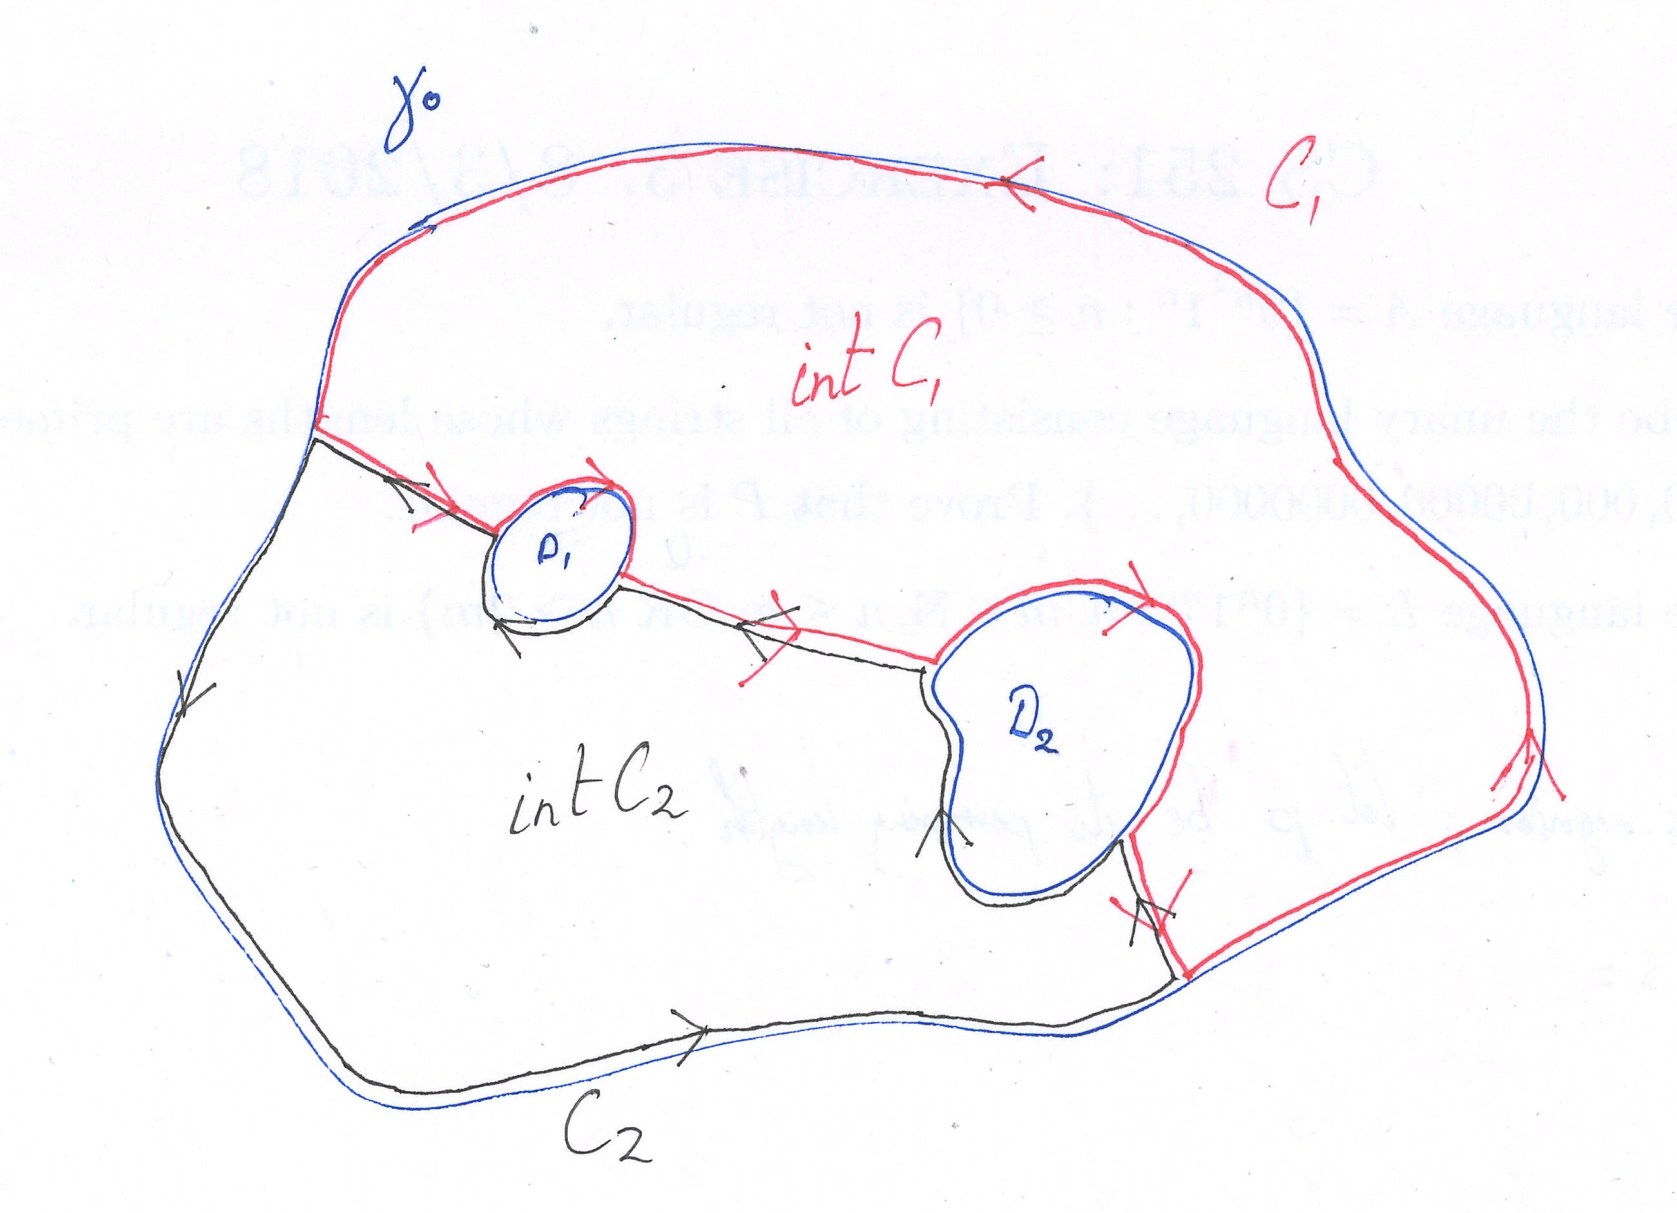
\includegraphics[width=.65\linewidth]{img/3_2_4-heur.png}
    \caption{Illustration de la justification heuristique}
    \label{3_2_4-heur}
\end{figure}

\[
D = \adh{D_0} \setminus \big(D_1 \cup D_2\big) = \adh{C_1} \cup \adh{C_2}
\]

Les bords de $\gamma_0, \gamma_1$ et $\gamma_2$ de $D_0,D_1$ et $D_2$ appartiennent à $D$.

\begin{itemize}
    \item 
    D'une part, $f$ holomorphe dans $\adh{C_1}$ et $\adh{C_2}$, $C_1$ et $C_2$ sont fermés $\xRightarrow[\textrm{Cauchy}]{\textrm{Thm.}}$
    
    \[\int_{C_1} f(z) \dz = 0 \textrm{ et } \int_{C_2} f(z) \dz = 0\]
    \item 
    D'autre part, avec $C_1$ et $C_2$ orientés positivement, on a:
    
    \[
    \int_{C_1} f(z) \dz + \int_{C_2} f(z) \dz = \int_{\gamma_0} f(z) \dz + \int_{\gamma_1} f(z) \dz + \int_{\gamma_2} f(z) \dz
    \]
    
    où $\gamma_0$ est orientée \textit{positivement} ($D_0$ à gauche), mais $\gamma_1$ et $\gamma_2$ orientées \textit{négativement} ($D_1$ et $D_2$ à droite).
\end{itemize}

Donc:

\[\int_{\gamma_0} f(z) \dz + \int_{\gamma_1} f(z) \dz + \int_{\gamma_2} f(z) \dz = 0\]

\begin{align*}
\implies \int_{\gamma_0} f(z) \dz &= - \int_{\gamma_1} f(z) \dz - \int_{\gamma_2} f(z) \dz \quad \textrm{orientation négative (dessin)}\\
&= \int_{\gamma_1} f(z) \dz + \int_{\gamma_2} f(z) \dz \quad \textrm{orientation positive (énoncé)}
\end{align*}


\section{Formule intégrale de Cauchy}

\subsection{Énoncé}

\begin{theorem}
    Soient $D \subset \C$ un domaine simplement connexe, $f: D \rightarrow \C$ une fonction holomorphe dans $D$ et $\gamma$ une courbe simple fermée régulière (par morceaux) orientée positivement contenue dans $D$.
    Alors:
    
    \[
    f(z) = \oipi \int_\gamma \frac{f(\xi)}{\xi - z} \dxi \quad \forall z \in \inte \gamma
    \]
\end{theorem}

\begin{illustration}
    $D = \C$
    
    Si $f$ est une fonction holomorphe dans $\C$, la valeur de la fonction $f$ en un point $z \in \C$ s'obtient en intégrant $\frac{f(\xi)}{\xi - z}$ le long de n'importe quelle courbe $\gamma$ (orientée positivement) telle que $z \in \inte \gamma$.
\end{illustration}

\subsection{Exemples d'utilisation}

\begin{example}[1]
    Soit $\gamma$ une courbe simple fermée régulière.
    Discuter en fonction de $\gamma$ la valeur de l'intégrale:
    
    \[\int_\gamma \frac{\cos 2z}{z} \dz\]
    
    Constatation: la fonction $g(z) = \frac{\cos 2z}{z}$ n'est pas définie en $z = 0$.
    
    Distinction de différents cas:
    
    \begin{description}
    \item[1\ier{} cas $0 \in \gamma$]
    L'intégrale n'est pas définie puisque $g(z) = \frac{\cos 2z}{z}$ n'est pas continue sur $\gamma$.
    
    \item[2\ieme{} cas $0 \notin \adh{\gamma}$]
    La fonction $g(z) = \frac{\cos 2z}{z}$ est holomorphe dans un domaine $D$ simplement connexe tel que $\adh{\gamma} \subset D$.
    Comme $\gamma \subset \adh{\gamma} \subset D$, alors le Thm. de Cauchy s'applique à la fonction $g$ et on trouve:
    
    \[\int_\gamma \frac{\cos 2z}{z} \dz = 0\]
    
    $\forall \gamma$ de ce type (i.e. $0 \notin \adh{\gamma}$).
    
    \item[3\ieme{} cas $0 \in \inte{\gamma}$]
    La fonction $f(\xi) = \cos 2\xi$ est holomorphe dans $\C$.
    Comme $\gamma \subset \C$, en lui appliquant la formule intégrale de Cauchy pour $z = 0$ (avec $D = \C$), on trouve:
    
    \[
    f(0) = \oipi \int_\gamma \frac{\cos 2\xi}{\xi - 0} \dxi
    \implies \int_\gamma \frac{\cos 2\xi}{\xi} \dxi = 2\pi i f(0) = 2\pi i \cos 0 = 2\pi i
    \]
    
    \textbf{Conclusion:} $\int_\gamma \frac{\cos 2z}{z} \dz = 2\pi i \quad \forall \gamma$ de ce type.
    \end{description}
\end{example}

\begin{remark}
    Pour le cercle unité de rayon $1$, on a $\gamma(\theta) = e^{i\theta}$ avec $\theta \in [0,2\pi[$, il faudrait calculer:
    
    \[
    \int_\gamma \frac{\cos 2z}{z} \dz
    = \int_0^{2\pi} \frac{\cos \big(2e^{i\theta}\big)}{e^{i\theta}} i e^{i\theta} \dth
    = i \int_0^{2\pi} \cos \big(2e^{i\theta}\big) \dth
    \]
\end{remark}

\begin{example}[2]
    Calculer
    
    \[\int_\gamma \frac{e^{z^2}}{z + i\pi} \dz\]
    
    où $\gamma$ est le cercle de rayon $4$ centré en $z = 1$.
    
    Utilisation de la formule de Cauchy, constatations:
    
    \begin{enumerate}[label=\arabic{enumi})]
    \item 
    La fonction $g(z) = \frac{e^{z^2}}{z + i\pi}$ n'est pas définie en $z = -i\pi$
    \item 
    $-i\pi \in \inte{\gamma}$
    \end{enumerate}

    On considère $\gamma$ orientée positivement et $f(\xi) = e^{\xi^2}$ qui est holomorphe dans $\C$.
    Formule intégrale de Cauchy pour $z = -i\pi$ (avec $D = \C$) donne:
    
    \[
    f(-i\pi) = \oipi \int_\gamma \frac{e^{\xi^2}}{\xi + i\pi} \dxi \implies \int_\gamma \frac{e^{\xi^2}}{\xi + i\pi} \dxi = 2\pi i f(-i\pi)
    \]
    
    Mais $f(-i\pi) = e^{(-i\pi)^2} = e^{-\pi^2}$, donc:
    
    \[\int_\gamma \frac{e^{z^2}}{z + i\pi} \dz = 2\pi i e^{-\pi^2}\]
    
    \textit{Autres exemples: ex. 1-4, série 6}
\end{example}

% !TeX spellcheck = fr_FR
\chapter{Séries de Laurent, pôles et résidus}


\section{Polynôme et série de Taylor d'une fonction holomorphe}

\subsection{Définitions et résultats}

\begin{hypothesis}
    Soit un ouvert $D \subset \Cx$ et $f: \begin{array}{ccc}
    D & \longrightarrow & \Cx\\
    z & \longmapsto & f(z)
    \end{array}$ une fonction holomorphe dans $D$ et $z_0 \in D$.
\end{hypothesis}

\begin{definition}
    Pour $N \in \N$, le \textbf{polynôme de Taylor} de $f$ de degré $N$ en $z_0$ est:
    
    \[
    T_N f(z) = \sum_{n = 0}^N \frac{f^{(n)}(z_0)}{n!}(z - z_0)^n
    \]
\end{definition}

\begin{result}[séries de Taylor]
    Soit $R > 0$ et $D_R(z_0) = \{z \in \Cx : \module{z - z_0} < R \}$ le plus grand disque de rayon $R$ centré en $z_0$ contenu dans $D$.
    
    Convention: si $D = \Cx \implies R = +\infty$ et $D_R(z_0) = \Cx$
    
    Alors:
    
    \begin{enumerate}[label=\arabic{enumi})]
        \item 
        \[
        T f(z) = \lim_{N \rightarrow +\infty} T_N f(z) = \sum_{n = 0}^{+\infty} \frac{f^{(n)}(z_0)}{n!}(z - z_0)^n
        \]
        
        existe et est finie $\forall z \in D_R(z_0)$. L'expression $T f(z)$ s'appelle \textbf{la série de Taylor} de $f$ en $z_0$.
        
        \item 
        De plus, on a $f(z) = T f(z) \quad \forall z \in D_R(z_0)$
        
        $R$ est appelé \textbf{le rayon de convergence} de la série de Taylor.
        
        \item 
        Les coefficients de la série de Taylor sont reliés à la formule de Cauchy par le corollaire du §3.4.
        On a:
        
        \[ \frac{f^{(n)}(z_0)}{n!} = \frac{1}{2\pi i} \int_\gamma \frac{f(\xi)}{(\xi - z)^{n+1}} \dxi \]
        
        où $\gamma \subset D_R(z_0)$ est une courbe simple fermée régulière orientée positivement telle que $z_0 \in \inte \gamma$.
    \end{enumerate}
\end{result}

\subsection{Exemples}

\begin{example}[1]
    \[f(z) = e^z\]
    
    est holomorphe dans $\Cx$.
    On a $f^{(n)}(z) = e^z$ et $f^{(n)}(0) = 1 \quad \forall n \in N$.
    
    Donc:
    
    \[ e^z = \sum_{n=0}^{+\infty} \frac{z^n}{n!} \quad \forall z \in \Cx \]
\end{example}

\begin{example}[2]
    \[f(z) = \frac{1}{1-z}\]
    
     est holomorphe dans $D = \Cx \setminus \{1\}$.
    
    Le plus grand disque centré en $z_0 = 0$ contenu dans $D$ est $D_1(0) = \{ z \in \Cx : \module{z} < 1 \}$.
    
    On a $f^{(n)}(z) = \frac{n!}{(1-z)^{n+1}}$ et $f^{(n)}(0) = n! \ \forall n \in \N$.
    
    Donc:
    
    \[
    \frac{1}{1-z} = \sum_{n=0}^{+\infty} z^n \quad \forall z \in \Cx, \module{z} < 1
    \]
    
    \textbf{\og Série géométrique \fg{}} avec rayon de convergence $R = 1$.
\end{example}

\begin{example}[3]
    \[f(z) = \frac{1}{1 + z^2}\]
    
    est holomorphe dans $D = \Cx \setminus \{-i; i\}$.
    
    Le plus grand disque centré en $z_0 = 0$ et contenu dans $D$ est $D_1(0) = \{z \in \Cx : \module{z} < 1\}$.
    
    On a:
    
    \[
    \frac{1}{1 + z^2}
    = \frac{1}{1 - \left(-z^2\right)}
    \overset{\textrm{Ex. 2}}{=}
    \sum_{n=0}^{+\infty} (-z^2)^n
    = \sum_{n=0}^{+\infty} (-1)^n z^{2n} \quad \forall z \in \Cx, \module{z} < 1
    \]
    
    Le rayon de convergence $R = 1$
\end{example}

\textit{Autre exemple: ex. 5, série 7}

\subsection{Applications}

\begin{enumerate}[label=\arabic{enumi})]
    \item Règle de l'Hôpital
    
    Soit $z_0 \in \Cx$ et $f, g$ deux fonctions holomorphes au voisinage de $z_0$ telles que $f(z_0) = 0$, $g(z_0) = 0$ et $g'(z_0) \neq 0$.
    Alors:
    
    \[ \lim_{z \rightarrow z_0} \frac{f(z)}{g(z)} = \lim_{z \rightarrow z_0} \frac{f'(z)}{g'(z)} = \frac{f'(z_0)}{g'(z_0)} \]
    
    \textit{Preuve: ex.4, série 8}
    
    \item Théorème de Liouville
    
    Soit $f: \Cx \rightarrow \Cx$ une fonction \textit{bornée} et holomorphe \textit{dans} $\Cx$, alors $f$ est constante.
    
    \textit{Preuve: corrigé de l'ex. 18, p.248 (§11.3)}
\end{enumerate}


\section{Développement et série de Laurent d'une fonction holomorphe}

\subsection{Problématique, définitions et résultats}


\begin{motivation}\hfill
    
    Le développement de Taylor d'une fonction $f$ donne une série en puissances \textbf{positives} de $z - z_0$ au voisinage d'un point $z_0$ où $f$ \textbf{est} holomorphe.
    
    \textbf{But:} généralisation avec un développement en puissances \textbf{positives} et \textbf{négatives} de $z - z_0$ où $z_0$ peut être une \textbf{singularité} de $f$.
\end{motivation}


\begin{hypothesis}\hfill
    
    Soit $D \subset \Cx$ un domaine simplement connexe, $z_0 \in D$ et $f: D \setminus \{z_0\} \rightarrow \Cx$ une fonction holomorphe dans $D \setminus \{z_0\}$.
\end{hypothesis}

\begin{definition}
    Pour $N \in \N$, le développement de Laurent de $f$ de degré $N$ au voisinage de $z_0$ est:
    
    \[ L_N f(z) = \sum_{n = -N}^{N} c_n (z - z_0)^n \]
    
    \[ = \frac{c_ {-N}}{(z - z_0)^N} + \ldots + \frac{c_ {-1}}{z - z_0} + c_0 + c_1 (z - z_0) + \ldots + c_n (z - z_0)^N \]
    
    avec
    
    \[ c_n = \oipi \int_\gamma \frac{f(\xi)}{(\xi - z_0)^{n + 1}} \dxi \]
    
    où $\gamma \subset D$ est une courbe simple fermée régulière (par morceaux) orientée positivement telle que $z_0 \in \inte \gamma$.
\end{definition}

\begin{result}
    Soit $R > 0$ et $D_R(z_0) = \{ z \in \Cx : \module{z - z_0} < R \}$ le plus grand disque de rayon $R$ centré en $z_0$ et contenu dans $D$.
    Alors:
    
    \begin{enumerate}[label=\arabic{enumi})]
        \item 
        \[ Lf(z) = \lim_{N \rightarrow \infty} L_N f(z) = \sum_{n = -\infty}^\infty c_n (z - z_0)^n \]
        
        existe et est finie pour tout $z \in D_R(z_0) \setminus \{z_0\}$.
        L'expression $Lf(z)$ s'appelle la \textbf{série de Laurent} de $f$ au voisinage de $z_0$.
        
        \item 
        De plus, on a $f(z) = Lf(z) \quad \forall z \in D_R(z_0) \setminus \{z_0\}$ et $R$ est appelé le \textbf{rayon de convergence} de la série de Laurent.
    \end{enumerate}
\end{result}

\begin{remark}\hfill
    
    \begin{enumerate}[label=\alph*)]
        \item 
        La série de Laurent de $f$ peut s'écrire sous la forme suivante:
        
        \[ Lf(z) = \sum_{n = -\infty}^{-1} c_n(z - z_0)^n + \sum_{n = 0}^{\infty} c_n(z - z_0)^n \]
        
        \begin{itemize}
        \item 
        La première série
        
        \[
        \sum_{n = -\infty}^{-1} c_n(z - z_0)^n =
        \sum_{n = 1}^{\infty} c_{-n}(z - z_0)^{-n} =
        \frac{c_{-1}}{z - z_0} + \frac{c_{-2}}{(z - z_0)^{-2}} + \ldots
        \]
        
        s'appelle la \textbf{partie singulière} de la série de Laurent.
        
        \item 
        La deuxième série
        
        \[
        \sum_{n = 0}^{\infty} c_n(z - z_0)^n =
        c_0 + c_1(z - z_0) + c_2(z - z_0)^2 + \ldots
        \]
        
        s'appelle la \textbf{partie régulière} de la série de Laurent.
        \end{itemize}

        \item 
        \textit{Si} $f: D \rightarrow \Cx$ est holomorphe en $z_0$, alors la série de Laurent coïncide avec la série de Taylor.
        
        En effet, la partie singulière de la série de Laurent est nulle puisque:
        
        Pour $n = 1, 2, 3, \ldots$, on a:
        
        \[ c_{-n} =  \oipi \int_\gamma \frac{f(\xi)}{(\xi - z_0)^{-n + 1}} \dxi
        = \oipi \int_\gamma f(\xi)(\xi - z_0)^{n - 1} \dxi
        = 0 \]
        
        par le Théorème de Cauchy (§3.2), car $f(\xi)(\xi - z_0)^{n - 1}$ est holomorphe dans $D$.
        
        Les coefficients de la partie régulière donnent la série de Taylor car:
        
        Pour $n = 1, 2, 3, \ldots$, on a:
        
        \[ c_{n} =  \oipi \int_\gamma \frac{f(\xi)}{(\xi - z_0)^{n + 1}} \dxi
        = \frac{f^{(n)}(z_0)}{n!}\]
        
        par le corollaire de la formule intégrale de Cauchy (§3.4), car $f(\xi)$ est holomorphe dans $D$.
    \end{enumerate}
\end{remark}

\subsection{Définitions issues de la série de Laurent}

\begin{definition}[1]
    $z_0 \in \Cx$ est un \textbf{point régulier} de $f \iff$ la partie singulière de la série de Laurent au voisinage de $z_0$ est nulle.
    
    C'est-à-dire:
    
    \[ Lf(z) = Tf(z) = \sum_{n = 0}^{\infty} \frac{f^{(n)}(z_0)}{n!} (z - z_0)^n \]
\end{definition}


























\begin{thebibliography}{9}
    \bibitem{mainbook} 
    Bernard Dacogna et Chiara Tanteri. 
    \textit{Analyse avancée pour ingénieurs}. 
    PPUR, 2017.
\end{thebibliography}

Toutes les références (numéro de théorème, définition, etc.) sont faites à ce livre.


\section*{Contributeurs}

\begin{itemize}
    \item Robin Mamie (IN)
    \item Eric Jollès (SC)
    \item Yves Zumbach (IN)
    \item Victor Cochard (IN)
    \item Ghali Chraibi (SC)
\end{itemize}
\end{document}